\begin{figure*}[!hbp]
    \centering
    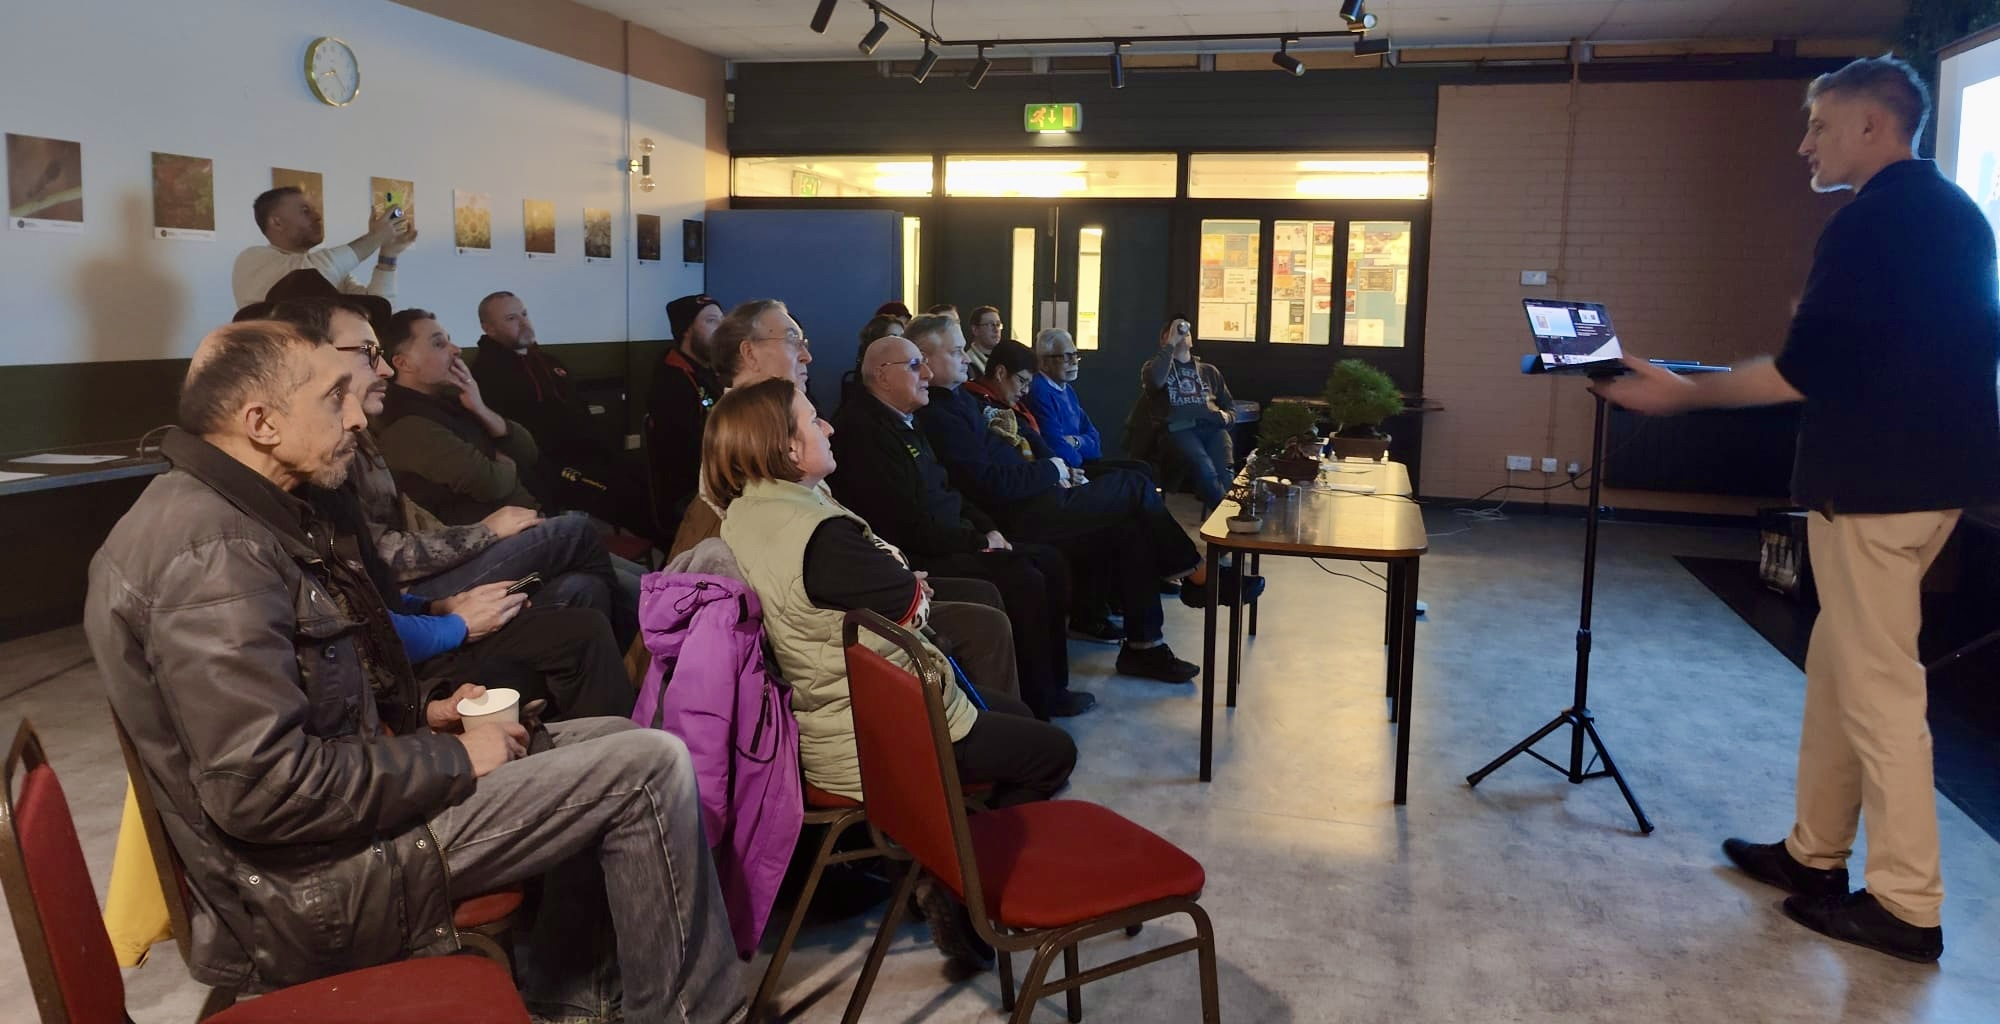
\includegraphics[width=1.0\textwidth]{2025_01/res/alex_rudd.jpg}
    \centerline{\emph{During the last meeting of the Twickenham Bonsai Club, Alex Rudd shared tips on selecting the perfect pot to enhance a bonsai.}}
\end{figure*}

\headline{{\textbf{\Large\sffamily The Perfect Match:}}\\
          {\textbf{\large\sffamily Choosing the Right Pot for Your Bonsai}}}
\label{2025-01-potting}
\noindent
In our January meeting, \textbf{Alex Rudd}, an experienced bonsai practitioner and founder of the \href{https://www.europeanbonsaipottercollective.com}{European Bonsai Potter Collective}, shared his expertise on the crucial art of selecting the perfect pot for your bonsai tree.
With his wealth of knowledge, Alex kept the audience hooked giving us a two\--hours deep dive into the nuances of this often overlooked aspect of bonsai care.
Here's a summary of his talk, packed with valuable insights for all bonsai enthusiasts.

\topic{Health Comes First}
\noindent
One of the most important takeaways from Alex's presentation was the idea that the \textbf{health of the tree} should always be the primary consideration when selecting a pot.
As Alex emphasised, the pot should never come before the tree's wellbeing.
If a tree is not yet ready for its final pot, pushing it into a pot too soon can be detrimental to its growth and health.
The tree's health is the foundation on which the aesthetic choices should be made.
Only once the tree is healthy and stable for a couple of years should we think about transferring it into its final pot.

\topic{The Role of the Pot in Aesthetics}
\noindent
After establishing the health of the tree as the top priority, Alex took us through a range of pot characteristics that contribute to the \textbf{aesthetic harmony} between the tree and its container.
The following aspects are essential in making a decision:

\begin{enumerate}
    \item \textbf{Glaze vs. Unglazed Pots}
    \begin{itemize}
        \item \textbf{Unglazed pots} are often best suited to \textbf{conifers} because of their rugged and earthy aesthetic, which complements the more austere nature of these trees.
        \item \textbf{Glazed pots}, on the other hand, tend to enhance the delicate leaves and colours of \textbf{deciduous trees}, bringing out their finer details.
    \end{itemize}

    \item \textbf{Shape, Size, and Proportions}
    \begin{itemize}
        \item \textbf{Shape:} Alex discussed how the shape of a pot should reflect the character of the tree. For instance, round pots often suit more delicate of \textbf{feminine} trees, while rectangular or square pots are typically associated with \textbf{masculine} trees, which have a more rugged, sturdy appearance. Pots with lobed shapes, reminiscent of flowers such as quince or lotus, occupy a middle ground between round and square forms in terms of perceived masculinity and femininity.

        \item \textbf{Size:} As a general rule, the width of the pot should be about \textbf{two-thirds the larger dimension of the tree} , unless the tree is a tall \textbf{literati style} (in which case, the pot may be smaller). The depth of the pot also affects the image of the tree – \textbf{deeper pots} tend to create a \emph{portrait} effect, focusing more on the tree's height, while \textbf{shallower pots} create a \emph{landscape} effect, making the tree appear more distant and part of a larger scene.
    \end{itemize}

    \item \textbf{Banding, Lips, and Feet}
    \begin{itemize}
        \item \textbf{Banding} plays a crucial role defining the \textbf{pot's personality}: deeper pots can often possess strong \textbf{masculine} characteristics that may clash with a desired \textbf{feminine} aesthetic in the tree, and vice versa. Horizontal banding helps to visually break down the pot's height, making it appear less imposing and more delicate. Conversely, embossed or protruding designs create vertical bands, which reinforce the pot's masculine character.

        \item The \textbf{lip}, or rim, of a pot significantly influences its character. A soft, curved lip lends a \textbf{feminine} feel, while a sharp, straight edge creates a more \textbf{masculine} impression. Furthermore, a lipless pot is generally better suited to trees displayed in a \emph{portrait style}, whereas a prominent lip tends to complement trees presented in a \emph{landscape style}.

        \item The \textbf{feet} of the pot are equally important. Raised feet often impart an air of sophistication, while a flatter, more practical foot is generally better suited to a more rugged tree.
    \end{itemize}

    \item \textbf{Colour and Painting}
    \begin{itemize}
        \item The \textbf{colour of the pot} plays a significant role in how the tree is perceived. Alex explained that \emph{conifers} often look best in \textbf{earthy, unglazed tones}, while \emph{deciduous trees} may benefit from contrasting or complementing pot colours that highlight their leaf colours and seasonal changes.

        \item Alex stressed that \textbf{contrast} can be more impactful than harmony in colour selection. For example, a yellow\--leafed tree may look stunning in a \textbf{green pot}, rather than one that matches the yellow leaves exactly.
    \end{itemize}
\end{enumerate}

\topic{Feminine vs. Masculine Pots}
\noindent
Throughout the talk, Alex continuously referred to the idea of \textbf{masculine and feminine pots}, which he believes is a crucial concept in achieving harmony between the tree and its pot.

\begin{itemize}
    \item \textbf{Masculine pots:} These tend to have \textbf{sharp} lines, \textbf{rectangular} shapes, and \textbf{deeper profiles}. They are ideal for trees that are \textbf{rugged}, \textbf{sturdy}, and have an \textbf{imposing presence}.

    \item \textbf{Feminine pots:} These are generally \textbf{rounded}, \textbf{shallow}, and feature more \textbf{curved lines}. They complement more \textbf{delicate} trees, often bringing out their \textbf{elegance} and \textbf{grace}.
\end{itemize}

The key is to choose a pot that complements the \textbf{character} of the tree, guided by a clear \textbf{vision} that takes into account its natural form and growth, ensuring a harmonious relationship that enhances the tree’s visual impact and reinforces its overall aesthetic appeal.

\topic{Rules Are Guidelines, Not Laws}
\noindent
While there are some established \textbf{guidelines} for choosing pots (such as proportions between height and width, matching the movement of the tree with the direction of the pot, and considering the tree's seasonal display), Alex was keen to stress that these rules are \textbf{not set in stone}.

The final selection should always come down to the \textbf{vision} or \textbf{message} the bonsai artist wants to convey to the viewer. Sometimes, breaking the rules can lead to a striking and personal choice that works beautifully. The important thing is to ensure that the pot \textbf{complements the aesthetic} of the tree, without causing \textbf{clashes} in form, colour, or style.

\topic{The Power of the Pot's Age and Growth}
\noindent
Alex also shared his experience with the \textbf{aging aspect} of bonsai pots, particularly in Japan, where pots are valued not only for their beauty but for the \textbf{patina} they develop over time. A pot with age tells a story and can enhance the overall look of an older tree. New pots, in contrast, may stand out too much, drawing attention away from the tree itself. Over time, a pot and its tree can grow together, with the pot gradually taking on characteristics that complement the maturing tree.

\topic{In Conclusion: Trust Your Instincts}
\noindent
While Alex highlighted the importance of understanding the technicalities of selecting a bonsai pot, he encouraged bonsai enthusiasts to also \textbf{trust their own instincts}. At the end of the day, it's your tree, your pot, and your creative vision. Feel free to break the rules when necessary and trust that your choices will evolve as you gain more experience with your trees.

As Alex Rudd puts it, \emph{``the most important thing is that you are satisfied with the image you're creating.''} If you love the pot and it works for your tree, that's all that truly matters.
\closearticle

\vfill
\begin{center}
	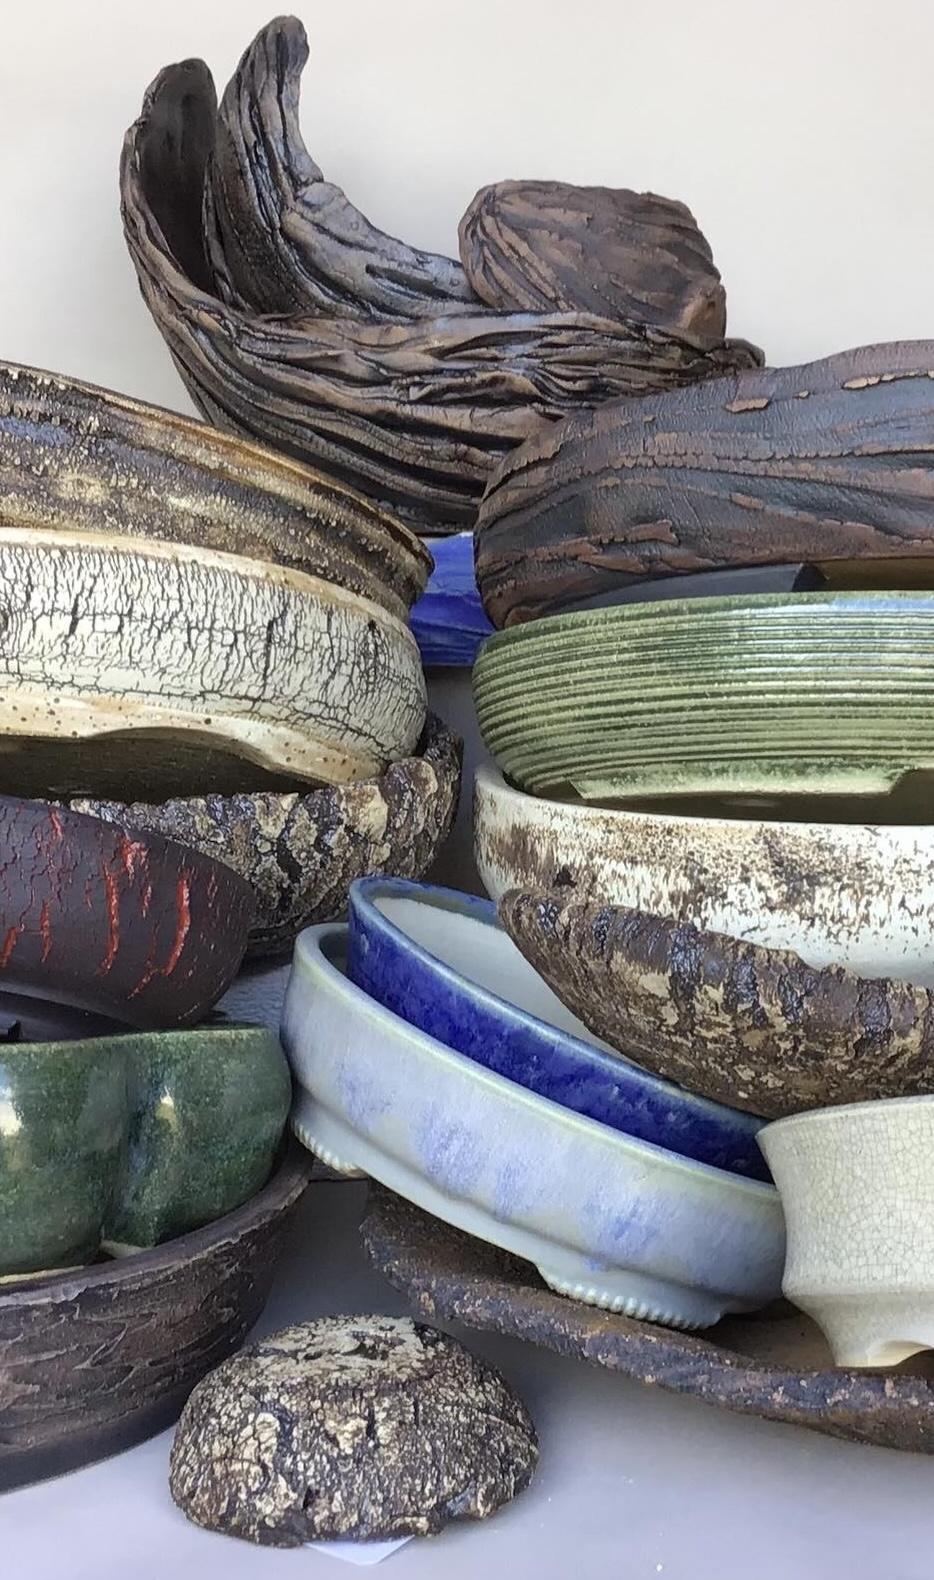
\includegraphics[width=0.95\columnwidth]{2025_01/res/pots}
\end{center}

\clearpage